%% This is an example first chapter.  You should put chapter/appendix that you
%% write into a separate file, and add a line \include{yourfilename} to
%% main.tex, where `yourfilename.tex' is the name of the chapter/appendix file.
%% You can process specific files by typing their names in at the 
%% \files=
%% prompt when you run the file main.tex through LaTeX.

% This is an example of how you would use tgrind to include an example
% of source code; it is commented out in this template since the code
% example file does not exist. To use it, you need to remove the '%' on the
% beginning of the line, and insert your own information in the call.
%
% \tagrind[htbp]{code/pmn.s.tex}{Code sample}{opt:pmn}


\chapter{Introduction} \label{ch:intro}

\section{Motivation} \label{ch:intro:motiv}

The fiber extrusion technology is known to have profound impact on the development of energy storage devices, synthetic polymers, wearable electronics, and many more \cite{synthetic, wearable_energy1, wearable_energy2}. Especially, optical fiber manufacturing has been an integral part of high-speed communication technology. In partnership with Sterlite Technologies Ltd. (hereinafter referred to as Sterlite), MIT's Device Realization Lab is innovating new approaches to improve the optical fiber extrusion process, specifically the controller design, simulation, tuning, and deployment process. A typical fiber draw tower in production is shown in Figure \ref{fig:tower}. 

\begin{figure}[hb!]
    \centering
    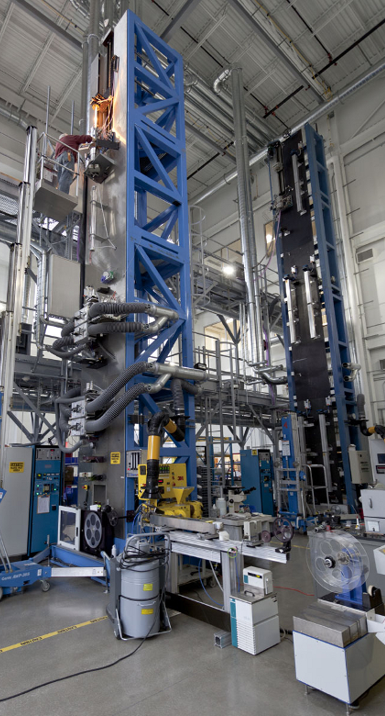
\includegraphics[width=0.5\textwidth]{figures/tower.png}
    \caption{Industrial optical fiber drawing tower on the production floor.}
    \label{fig:tower}
\end{figure}

There are many challenges in deploying new controllers to established, industrial-grade equipment. One of the challenges is to choose an appropriate method to develop an adequate model to explain the inner workings of the aggregate processes and controllers. There are three methods by which such models are created, 
\begin{enumerate}
    \item \textbf{White-box models}, which necessitate complete insight into the underlying physics to develop a model; 
    \item \textbf{Black-box models}, which require no knowledge of the internal structure and are developed solely on input-output data;
    \item \textbf{Grey-box models}, which are hybrids of the two approaches above, combining measured data and partially represented physics.
\end{enumerate}

Another challenge resides in tuning multiple controllers while obeying their limited operational design domain. Conventionally, controller tuning in the production plant is done in an isolated, trial-and-error fashion – make a small tweak to one of the parameters, examine the output, rely on intuition to consider the next tuning parameter, and repeat until performance is satisfied. The disadvantage of this approach is apparent; aside from the time- and labor- intensiveness of the process, mechanical systems often have practical constraints for safety measures (e.g. actuator limits, ramp rate, etc), which prevent the system from receiving any arbitrary control input \cite{constraints}. Using this approach, in order to simultaneously develop multiple controllers to achieve production quality, system integration may require multiple design and debugging iterations. Such modifications often lead to unnecessary downtime in production and monetary costs in research and development. 

This research project presents a data-driven approach to model nonlinear system dynamics and highlights the implementation in active optical fiber manufacturing processes, for which limited experimentation is possible. The need for better controllers is driven by the goals of reduced production variation and quicker recovery from production defects. A procedure to verify product performance and deploy systems to production is also provided as a recommendation. 

\section{Optical Fiber Extrusion Process}\label{ch:intro:fiber}

\begin{figure}[ht!]
    \centering
    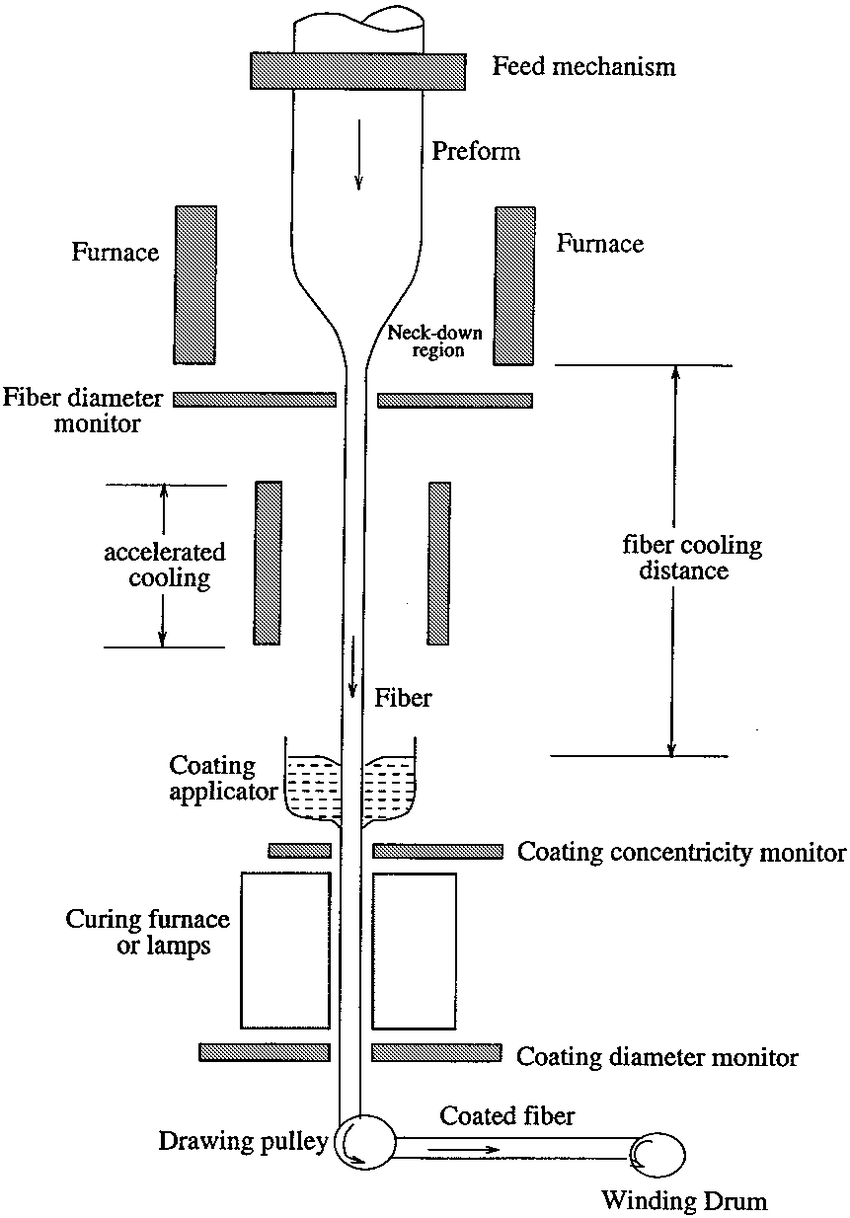
\includegraphics[width=0.75\textwidth]{figures/neckdown.png}
    \caption{A simplified illustration of a typical optical fiber drawing tower and its components \cite{neckdown}.}
    \label{fig:neckdown}
\end{figure}

A typical optical fiber drawing tower is illustrated in Figure \ref{fig:neckdown}. The fiber extrusion system in this study employs a thermal drawing technique. The process begins with a cylindrical preform rod, which is made of optical glass, being fed into a radiative furnace. The preform becomes heated and malleable, which enables it to form the neck-down profile axially and flow from a preform diameter of a few centimeters to optical fiber of micron-level diameter \cite{neckdown}. A supply of helium gas is injected into the furnace to cool down and solidify the glass fiber. The capstan assembly at the bottom pulls it with a specified tension force and velocity to produce the finished product, a spool of fiber wounded up at the end of the process. Multiple sensors also work to monitor the real-time states of the fiber drawing system, among which are the temperature of the furnace, bare fiber diameter (BFD), and velocity and tension at the capstan pulley. 

\begin{figure}[ht!]
    \centering
    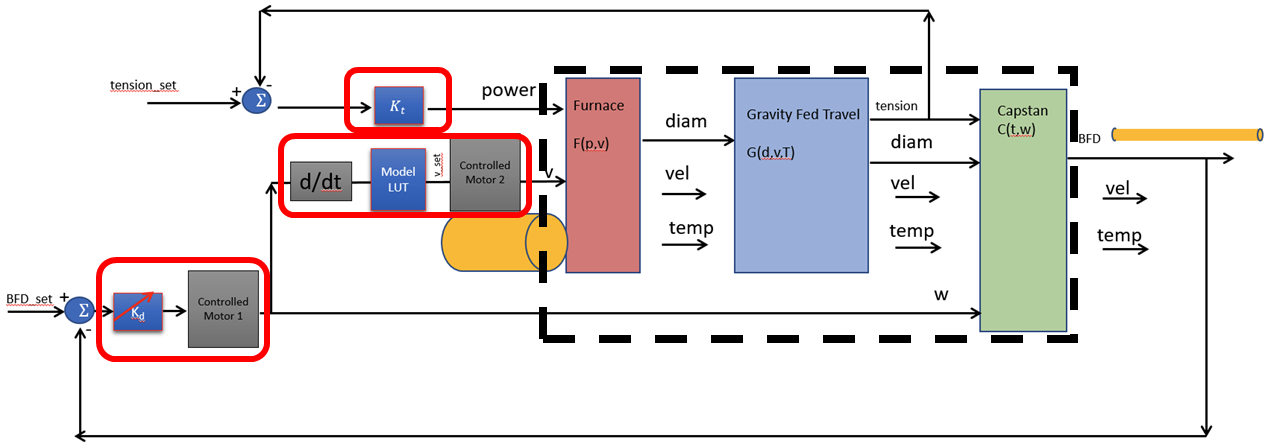
\includegraphics[width=\textwidth]{figures/stl_system_diag.png}
    \caption{Schematic diagram of the optical fiber drawing system from Sterlite Technologies Ltd. The red solid boxes indicate the three controllers, and the black dashed box indicates the aggregate fiber drawing plant to be identified.}
    \label{fig:stl_system_diag}
\end{figure}

A schematic diagram of Sterlite's fiber drawing system is shown in Figure \ref{fig:stl_system_diag}. There are three controllers modulating the signals involved in the fiber extrusion process. The tension controller, labeled as $K_t$ in Figure \ref{fig:stl_system_diag}, is a Proportional-Integral-Derivative (PID) controller that takes the error in measured tension as input and outputs the power signal to the radiative furnace. The diameter controller, labeled as $K_d$ in Figure \ref{fig:stl_system_diag}, is also a PID controller that takes the error in BFD and has capstan speed as its output. The preform velocity controller (the middle red box in Figure \ref{fig:stl_system_diag}) involves a discrete lookup table that correlates the slope of the capstan speed (i.e. acceleration) to the feed speed of the preform. Tension force during the neck-down process and the real-time BFD are measured by sensors for feedback control. 

\section{Previous Work}

There is an ample amount of literature investigating fiber manufacturing systems. The fluid dynamics and heat transfer problems involved in the fiber drawing process are well-studied; its governing equations can be derived from constitutive relations and fundamental conservation laws \cite{fiber_fluids1,fiber_fluids2,fiber_fluids3,fiber_fluids4}. The control problems of process variables (e.g. temperature of molten glass, winding speed, ambient temperature, etc) are also formulated \cite{fiber_ctrl1, fiber_ctrl2}. However, most controller design studies in the manufacturing field are developed from first principles \cite{manu_ctrl1, manu_ctrl2, manu_ctrl3}; the data-driven approach to controller design has yet to be fully explored. 

In addition, David Donghyun Kim developed a desktop fiber manufacturing system as part of his doctoral research in MIT's Device Realization Lab \cite{ddkim_phdthesis}. The implication of this system is threefold: 
\begin{enumerate}
    \item To gather measurement data that mimic the fiber extrusion process in production;
    \item To serve as a research platform for prototyping low-cost components and manufacturing techniques;
    \item To provide educational value to teach fundamentals on manufacturing, feedback controls, machine learning, and more.
\end{enumerate}

In addition, Sangwoon Kim also developed a deep reinforcement learning approach for tracking control of the fiber extrusion process, implemented with the desktop prototyping hardware \cite{sangwoon}. Although this thesis concerns about the full-scale, production-grade fiber draw tower in Sterlite, the approach for modeling and simulating the process dynamics can be applicable to the prototyping hardware, which can be used as a validation tool as well.  


\section{Thesis Overview}\label{ch:intro:thesis_ov}

This thesis details the development of models for the aggregate plant (i.e. the black box in Figure \ref{fig:stl_system_diag}) and each of the controllers (i.e. the red boxes in Figure \ref{fig:stl_system_diag}) in the optical fiber drawing system. 

The process dynamics of the aggregate plant is modeled with a black-box, neural network approach. The fiber extrusion process involving the radiative furnace, gravity fed travel, and the capstan assembly is treated as a black box, since it can be collectively described by a set of heat transfer and fluid dynamics equations. The input-output relationship of the black-box system is obtained by training neural networks of various configurations. Chapter \ref{ch:ml} presents the theoretical background of Long Short-Term Memory (LSTM) neural networks and machine learning in general. Chapter \ref{ch:exp} describes the experiments conducted to obtain said black-box correlation, and our metric to verify the model's generalizability and robustness. 

The modeling and simulation for the three controllers, mentioned in Section \ref{ch:intro:fiber}, are developed using statistical time-series system identification methods, namely Output-Error (OE) and AutoRegressive Moving Average model with eXogenous inputs (ARMAX). Chapter \ref{ch:sysid} details the theoretical background for these methods, the procedure by which a model's orders and parameters are determined, and the evaluation criteria that selects a model for simulation. The results of the identification process on the bare fiber diameter controller are also presented as a comprehensive case study.

The closed-loop simulation connecting all components of this work is found in Chapter \ref{ch:res}, along with a discussion on explainability of neural networks and time-series models through the lens of classical control. The implications of this work are also discussed, namely the usability of the closed-loop simulation as a design tool for controller improvements. This thesis ends with a discussion admitting the limitations of this work and a conclusion enumerating the potential areas that warrant further research in this ongoing project. 

% \begin{eqnarray*}
% a_i & = & a_j + a_k \\
% a_i & = & 2a_j + a_k \\
% a_i & = & 4a_j + a_k \\
% a_i & = & 8a_j + a_k \\
% a_i & = & a_j - a_k \\
% a_i & = & a_j \ll m \mbox{shift}
% \end{eqnarray*}
% instead of the multiplication.  For example, you could use:
% \begin{eqnarray*}
% r & = & 4s + s\\
% r & = & r + r
% \end{eqnarray*}
% Or by xx:
% \begin{eqnarray*}
% t & = & 2s + s \\
% r & = & 2t + s \\
% r & = & 8r + t
% \end{eqnarray*}
